
\begin{appendix}
\section{Sistema vuoto-azoto}
Molto spesso in chimica si ha la necessità di svolgere reazioni in assenza di gas atmosferici come ossigeno, azoto, anidride carbonica e/o acqua; questa necessità può essere per il chimico una vera e propria sfida. Negli anni sono state sviluppate numerose tecniche per allontanare gli interferenti atmosferici dall'ambiente di reazione. Ai giorni d'oggi alternativa forse più semplice e pratica rimane la tecnica Schlenk. Come mostrato in \autoref{fig:schlenk} il sistema di Schlenk, detto anche sistema vuoto azoto, è composto principalmente da una pompa e un insieme di valvole che permettono la creazione di vuoto e l'immissione di gas inerte (in questo caso azoto) senza che i gas presenti in atmosfera entrino a contatto con il sistema. L'apparato presenta una valvola a 3 vie che collega una linea di valvole o alla bombola di immissione dell'azoto o alla pompa a vuoto. Il passaggio tra il vuoto e l'azoto deve essere svolto in modo tale da non collegare con la valvola il sistema di vuoto con la sorgente di gas. Si noti come nel sistema è presente un resevoir per l'azoto liquido nel quale è immerso il tubo a U che collega il sistema di valvole con la pompa, ciò viene fatto per evitare che gas condensabili, potenzialmente dannosi per la pompa, possano essere aspirati. 


\begin{figure}[h! ]
    \centering
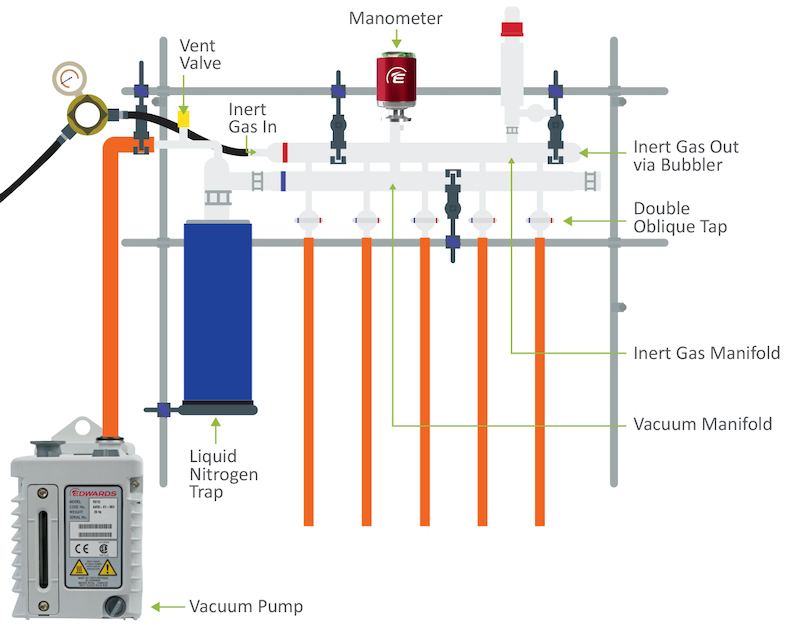
\includegraphics[width=0.6\linewidth]{Relazione/foto/Schlenk lines diagram.jpg}
    \caption{Schema sistema vuoto azoto}
    \label{fig:schlenk}


\end{figure}

Il sistema viene protetto dalle possibili sovrappressioni da un gorgogliatore immerso in paraffina che permette la fuoriuscita del gas in eccesso impedendo nello stesso tempo ai gas presenti all'esterno di entrare nell'apparato. Prima dell'effettivo utilizzo bisogna rendere il sistema completamente saturo di gas inerte rimuovendo così l'aria presente; ciò viene svolto facendo dei cicli di vuoto-azoto con il sistema chiuso. Una volta bonificato il sistema si procede a saturare tutto di azoto e al collegamento dei tubi alla vetreria codata usata per la sintesi, si procede un'altra volta con cicli vuoto azoto per rimuovere anche ogni traccia di inquinanti dall'apparato completo. Le ulteriori modifiche o le eventuali aggiunte di reagenti andranno svolte in pressione positiva di azoto o tramite setto poroso in modo da lasciare il sistema quanto più libero da inquinanti che potrebbe inficiare sul risultato della procedura che cerchiamo di replicare. Ogni pezzo di vetreria deve essere prontamente ingrassato per evitare l'infiltrazione di gas; per questo compito si utilizza del grasso al silicone. Gli apparati di filtrazione e reazione mostrati nelle sezioni precedenti sono stati tenuti insieme da elastici. Limmissione e l'aspirazione di gas sono state fatte dalla valvola più lontana dal contenitore dove sono contenuti i reagenti.
\clearpage
\section{Dati e tabelle}
\label{sec:dati}
\subsection{Tabelle}
In questa sezioni sono presente tutte le informazioni notate usate per i calcoli\footnote{I dati di densità sono stati presi dall'etichette delle bottiglie o dal sito SigmaAldrich}.
\begin{table}[ht!]
    

\textbf{Densità \hspace{8mm}}
\vspace{1mm}
\begin{tabular}{l c}
\hline Composto & Densità $[\mathrm{g} / \mathrm{mL}]$\\
\hline\hline en & 0.899 \\
\ce{Et2en} & 0.827 \\
$\mathrm{HCOH}$ & 1.09 \\
$\mathrm{CH}_3 \mathrm{NO}_2$ & 1.127 \\
$\mathrm{P}(\mathrm{OPh})_3$ & 1.184 \\
Aldeide Salicilica & 1.146 \\
\hline
\end{tabular}

\end{table}
\begin{table}[ht!]
  \vspace{1mm}  
\textbf{Massa molare}
\begin{tabular}{ l c }
\hline Composto & Massa molare $[\mathrm{g} / \mathrm{mol}]$ \\
\hline\hline 
 \ce{NiCl2}& 129.6 \\

$\mathrm{NiCl}_2 \cdot 6 \mathrm{H}_2 \mathrm{O}$ & 237.70 \\
 $\mathrm{NiBr}_2 \cdot 3 \mathrm{H}_2 \mathrm{O}$ & 272.55 \\
\ce{[Ni(NH3)6]Cl2}& $231.78 $
 \\ $\left[\mathrm{Ni}\left(\mathrm{Et}_2 \mathrm{en}\right)_2\left(\mathrm{H}_2 \mathrm{O}\right)_2\right] \mathrm{Br}_2$ & 486.93 \\
$\left[\mathrm{Ni}\left(\mathrm{Et}_2 \mathrm{en}\right)_2 \mathrm{Br}_2\right]$ & 450.90 \\
 $\mathrm{CoCl}_2 \cdot 6 \mathrm{H}_2 \mathrm{O}$ & 237.93 \\
$\left[\mathrm{Co}(\mathrm{en})_3\right] \mathrm{Cl}_3$ & 345.58 \\
$\left[\mathrm{Ni}(\mathrm{en})_3\right] \mathrm{Cl}_2 \cdot 2 \mathrm{H}_2 \mathrm{O}$ & 345.92 \\
en & 60.10 \\
 $\mathrm{Et}_2 \mathrm{en}$ & 116.20 \\
$[\mathrm{Co}($ dinosar $)] \mathrm{Cl}_3$ & 539.73 \\
$\mathrm{Co}\left(\mathrm{NO}_3\right)_2 \cdot$ 6\ce{H2O} & 291.03 \\
 $\mathrm{CH}_3 \mathrm{NO}_2$ & 61.04 \\
 $\mathrm{P}(\mathrm{OPh})_3$ & 310.28 \\
 $\mathrm{HCo}\left[\mathrm{P }(\mathrm{OPh})_3\right]_4$ & 1301.02 \\
 
 $\mathrm{HCOH}$ & 30.03 \\

 \ce{WO3}  & 231.84 \\

 \ce{Co(salen)} &  
325.23 \\
 \ce{Cr2(OAc)4 2.H2O } &  788.40 \\
 \ce{K2Cr2O7 } &  294.19 \\
  \ce{Zn } &  	65.41 \\
  Aldeide Salicilica & 	122.12 \\
  \ce{NaBH4} &37.83\\
\hline
\end{tabular}

\end{table}
\clearpage
\subsection{Dati raccolti}


\begin{table}[ht!]
    

\textbf{Provette}
\vspace{1mm}
\begin{tabular}{lcc}
\hline Composto & Massa finale $[\mathrm{g}] $ & Tara $[\mathrm{g}]$ \\
\hline\hline 
$\left[\mathrm{Ni}(\mathrm{en})_3\right] \mathrm{Cl}_2 \cdot 2 \mathrm{H}_2 \mathrm{O}$ & 19.4424  & 15.1714\\
\ce{[Ni(NH3)6]Cl2}& 17.7280 & 15.1515
 \\ $\left[\mathrm{Ni}\left(\mathrm{Et}_2 \mathrm{en}\right)_2\left(\mathrm{H}_2 \mathrm{O}\right)_2\right] \mathrm{Br}_2$ & 17.1101 & 15.0134 
 \\ $\left[\mathrm{Ni}\left(\mathrm{Et}_2 \mathrm{en}\right)_2 \mathrm{Br}_2\right]$ tappo & 21.6770 & 21.6120 \\
$\left[\mathrm{Ni}\left(\mathrm{Et}_2 \mathrm{en}\right)_2 \mathrm{Br}_2\right]$ & 15.8230 & 15.0129  \\

$\left[\mathrm{Co}(\mathrm{en})_3\right] \mathrm{Cl}_3$ $\#1$ & 19.2535 & 15.1411 \\
$\left[\mathrm{Co}(\mathrm{en})_3\right] \mathrm{Cl}_3$ $\#2$ & 18.9275 & 15.1711 \\

$[\mathrm{Co}($ dinosar $)] \mathrm{Cl}_3$ & 17.7611 & 15.0861 \\ $\mathrm{HCo}\left[\mathrm{P }(\mathrm{OPh})_3\right]_4$ & 15.6794 & 15.0190 \\
 \ce{Co(salen)} & 18.8692 & 15.1226\\
 \ce{[Cr2(OAc)4].2H2O } & 17.6259 & 15.0654\\
 
\hline
\end{tabular}

\end{table}


\begin{table}[ht!]
\textbf{Misure magnetiche}
\vspace{1mm}
\begin{tabular}{lccc}
 \hline 
 Composto & Altezza [cm] & Massa$[\mathrm{g}] $ & Misura   \\
\hline\hline 
 \multirow{4}{*}{$\left[\mathrm{Ni}\left(\mathrm{Et}_2 \mathrm{en}\right)_2\left(\mathrm{H}_2 \mathrm{O}\right)_2\right] \mathrm{Br}_2$} & 3.0 & 1.7547 & 93\\ 

& 3.4 & 1.7714 & 109 \\
& 2.6 & 1.7529 & 108 \\
& 2.9 & 1.7598 & 110 \\

\hline
 \multirow{4}{*}{ \ce{[Ni(en)3]Cl2}} & 2.7 & 1.7426 & 98 \\ 
 & 3.2 & 1,7515 & 98 \\
& 3.4 & 1,7551 & 99 \\
& 2.7 & 1.7423 & 97 \\


 
\hline
\end{tabular}

\caption{La massa della provetta utilizza è 1.6929 g, mentre il valore fornito dallo strumento per la provetta vuota è -65.}
\label{tab:magnet}
\end{table}
\begin{table}[ht!]
\textbf{Pesate}
\vspace{1mm}
\begin{tabular}{lc}
\hline Composto & Massa finale $[\mathrm{g}] $ \\
\hline\hline 
 $\left[\mathrm{Ni}\left(\mathrm{Et}_2 \mathrm{en}\right)_2\left(\mathrm{H}_2 \mathrm{O}\right)_2\right] \mathrm{Br}_2$ & 0.8751\\ 

 \ce{[Co(en)3]Cl3} & 2.450 \\
 
 
\ce{[Ni(NH3)6]Cl2}  & 
1.1532\\
 \ce{[Ni(en)3]Cl2.2H2O}& 1.7250\\
   \ce{[Ni(Eten)2 2H2O]Br2}&0.4521\\
\hline
\end{tabular}

\caption{Risultati pesate}
\label{tab:pesate}
\end{table}


\begin{table}[ht!]
    \textbf{Misure di conducibilità}
    \begin{tabular}{l c c }
   Composto  & Massa[g] & Resistenza[$\Omega$] \\
   \hline\hline
       \ce{H_xWO3}  &  0.247 & 2.1 \\
        \ce{H_xWO3} trattato & 0.233  & $9 \cdot 10^5$\\
        \hline
    \end{tabular}
    \caption{Risultati prove di conducibilità}
    \label{tab:conduci}
\end{table}




\clearpage
\section{Spettri completi}

\begin{figure}[h!]
    \centering
    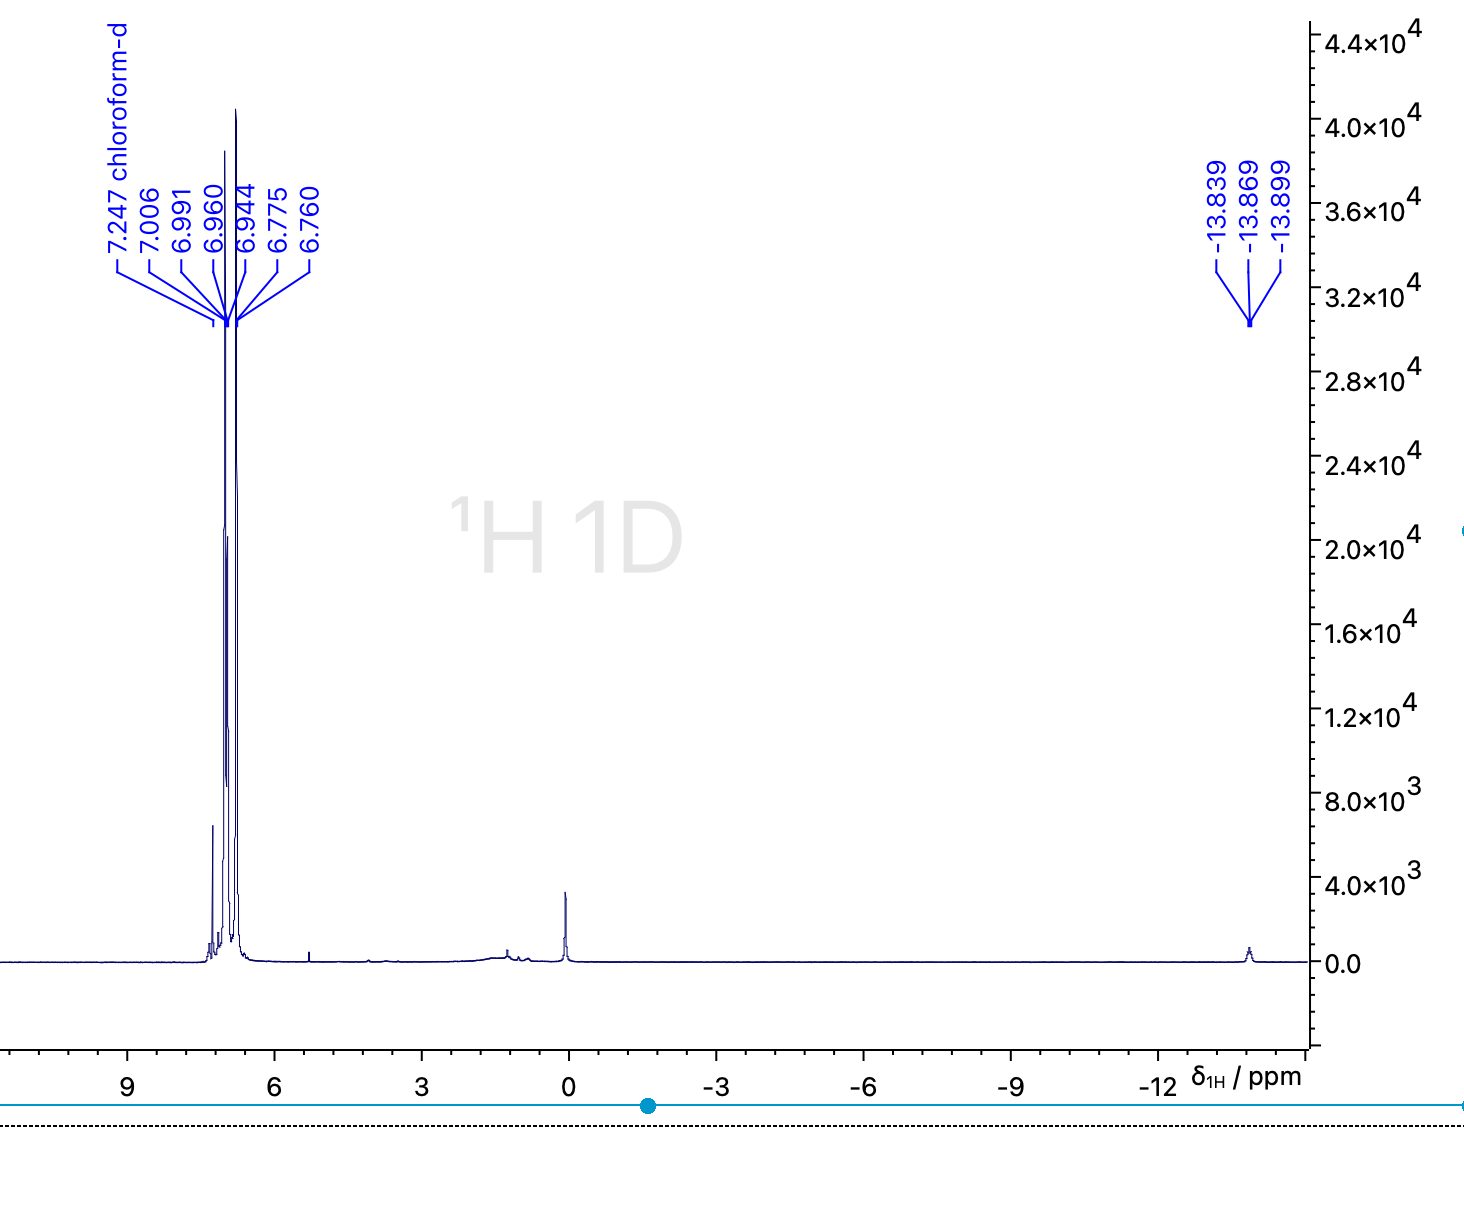
\includegraphics[width=\linewidth]{Relazione/foto/CoH_peak_calcall.png}
    \caption{ Spettro H-NMR
    $\ce{HCo(OPPh3)4 }$ }
    \label{fig:cohfull}
\end{figure}


\begin{figure}[h!]
    \centering
    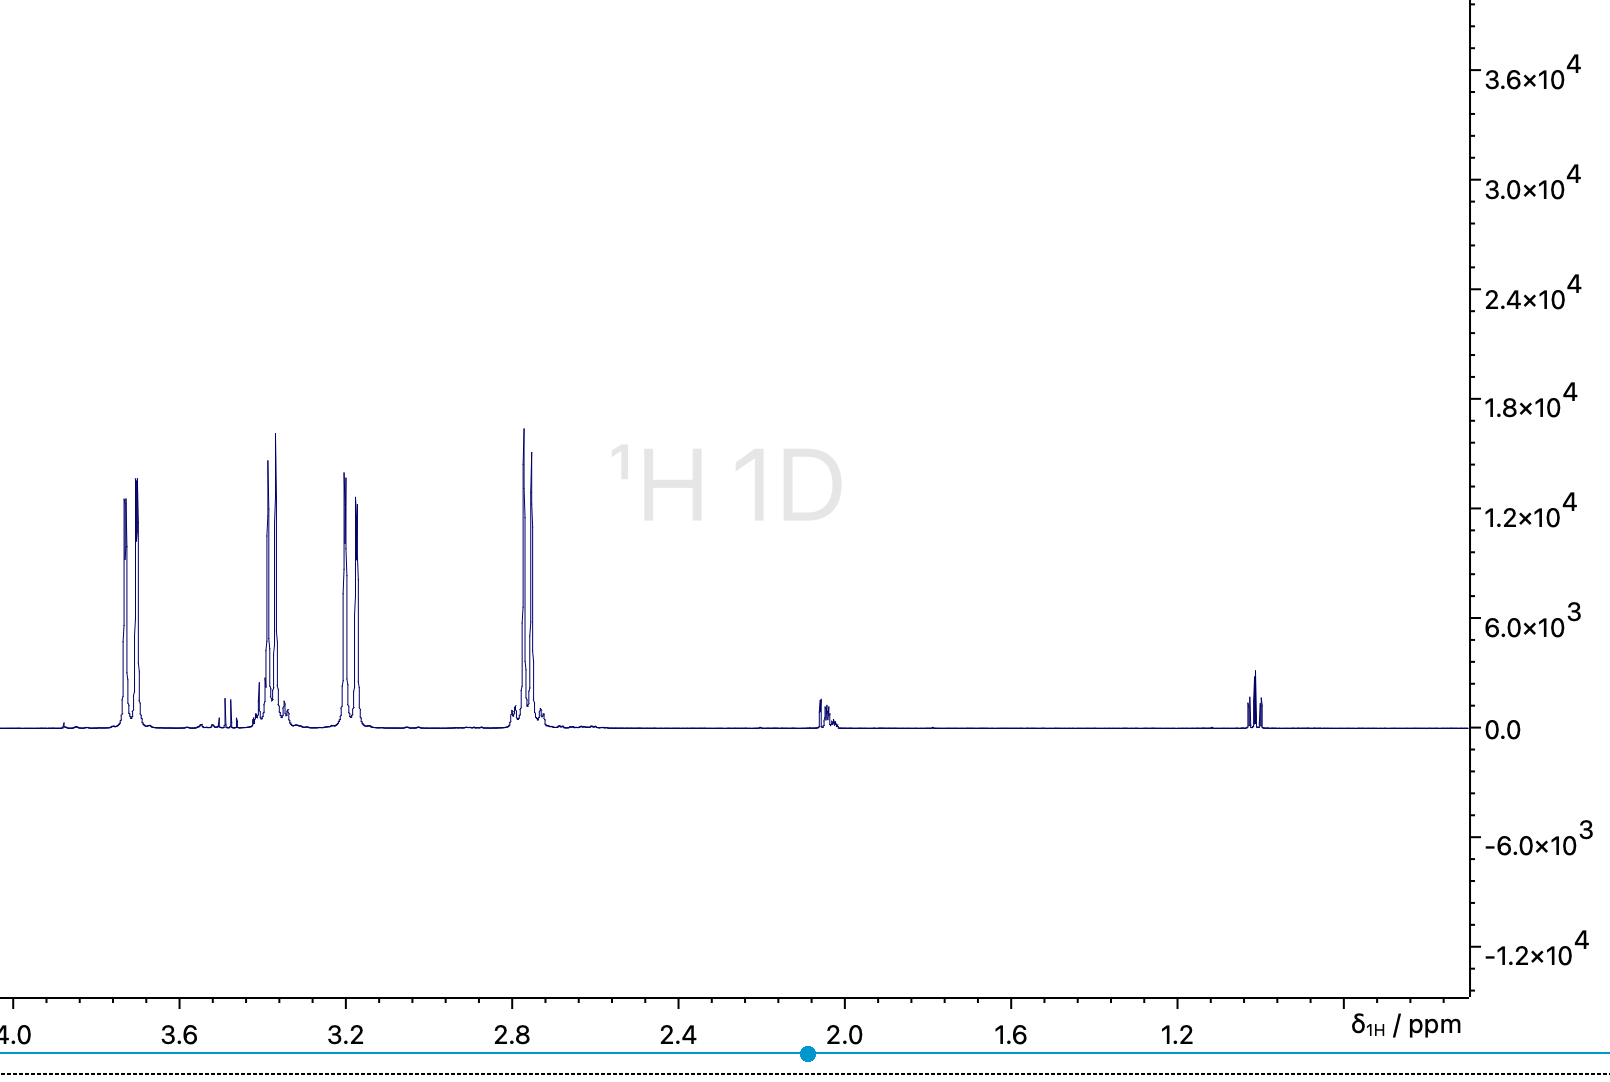
\includegraphics[width=\linewidth]{Relazione/foto/Dinosar_full.png}
    \caption{Spettro H-NMR Co(dinosar)}
    \label{fig:cohfull}
\end{figure}



\clearpage
\section{Raccolta foto}


\begin{figure}[h!]
\centering
\begin{tabular}{|c|c|}
\hline
\subf{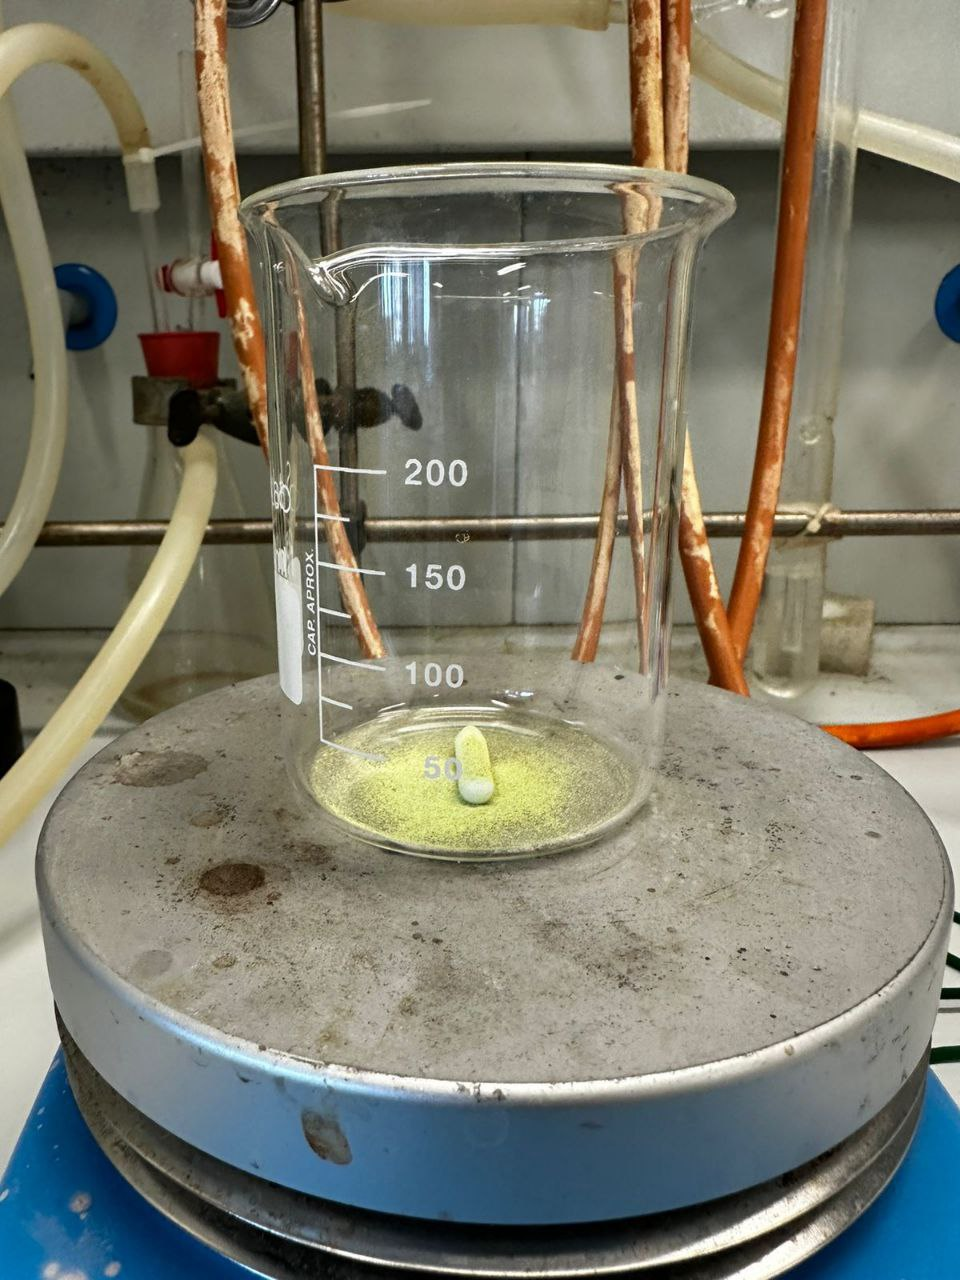
\includegraphics[width=60mm]{Relazione/foto/photo_2023-12-22 14.57.40.jpeg}}
     {\ce{WO3} prima dell'aggiunta di zinco}
&
\subf{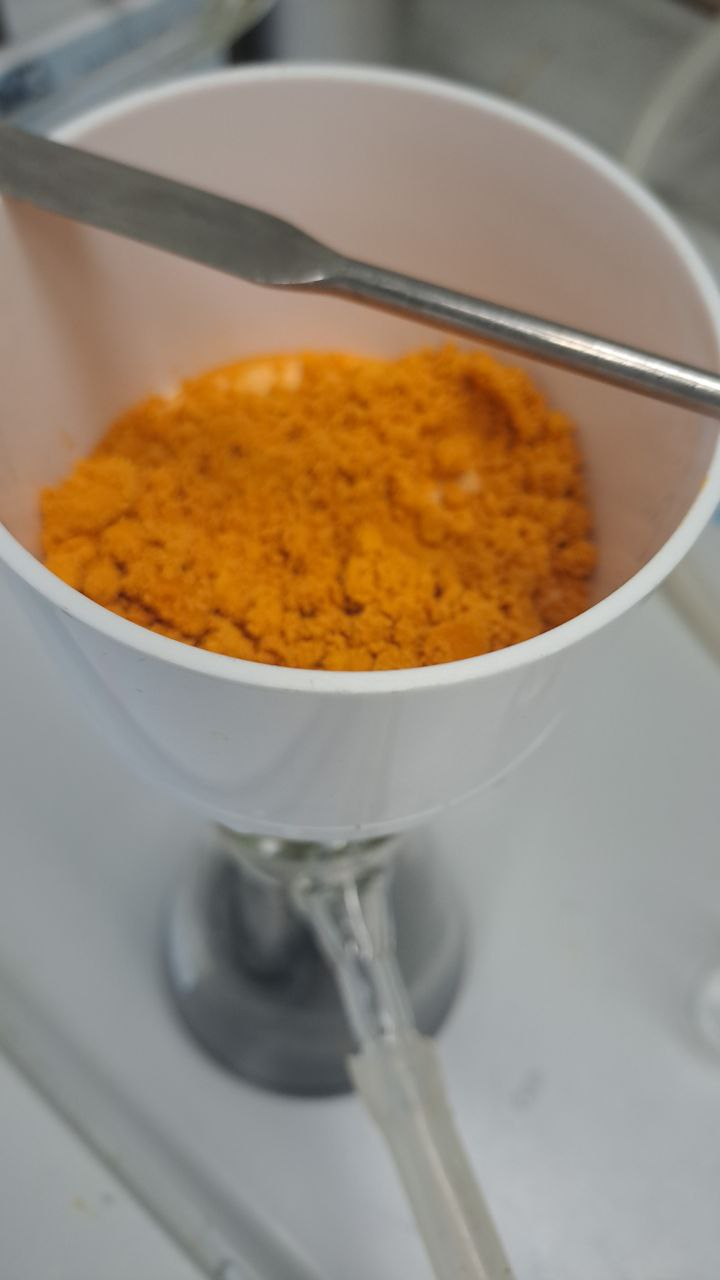
\includegraphics[width=50mm]{Relazione/foto/photo_2023-12-22 14.58.06.jpeg}}
     {\ce{[Co(en)3]Cl3}}
\\
\hline
\subf{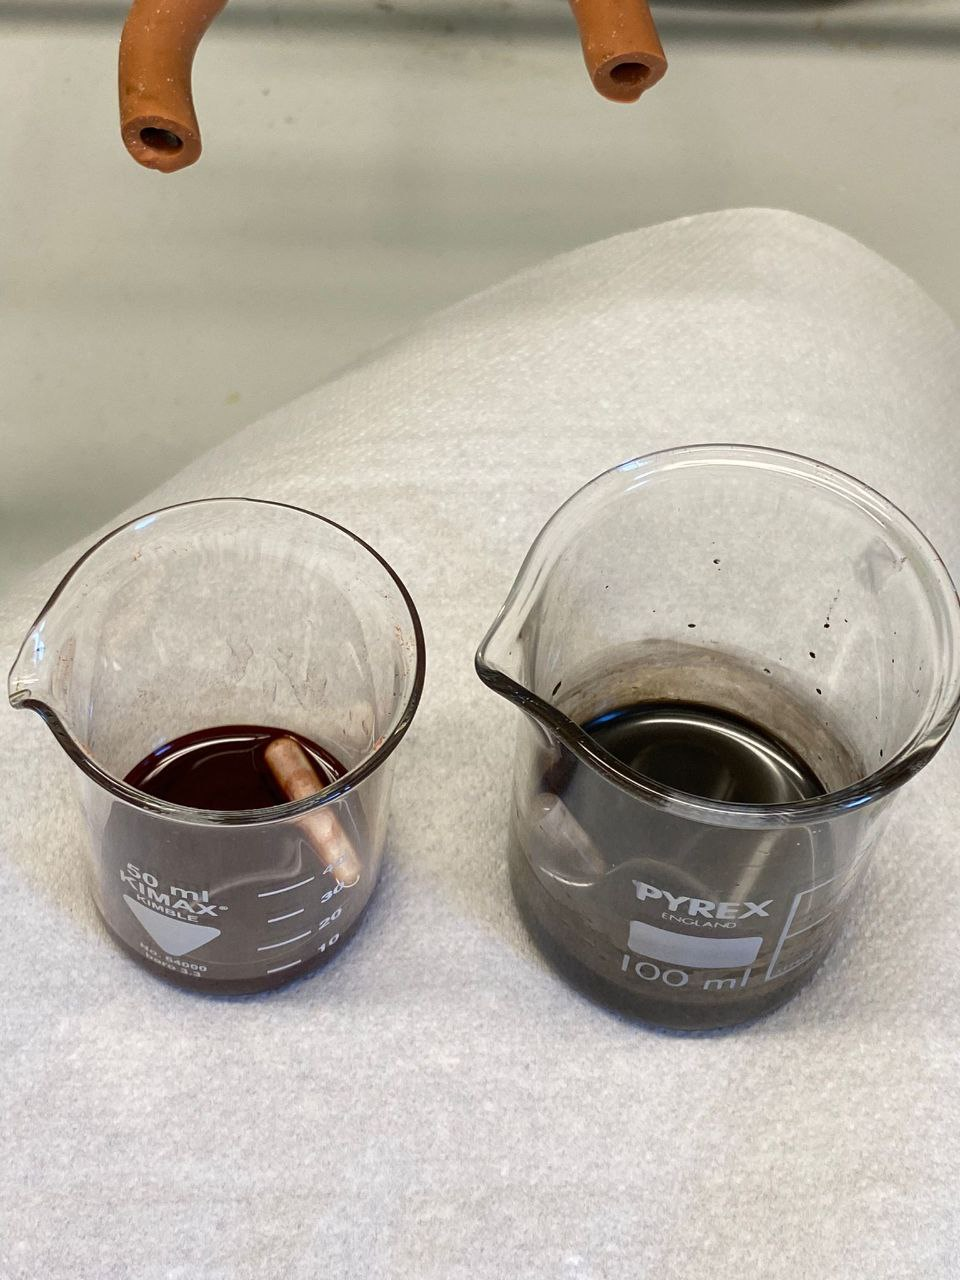
\includegraphics[width=60mm]{Relazione/foto/photo_2023-12-22 14.58.08.jpeg}}
     {Co(salen) ossigenato e non ossigenato}
&
\subf{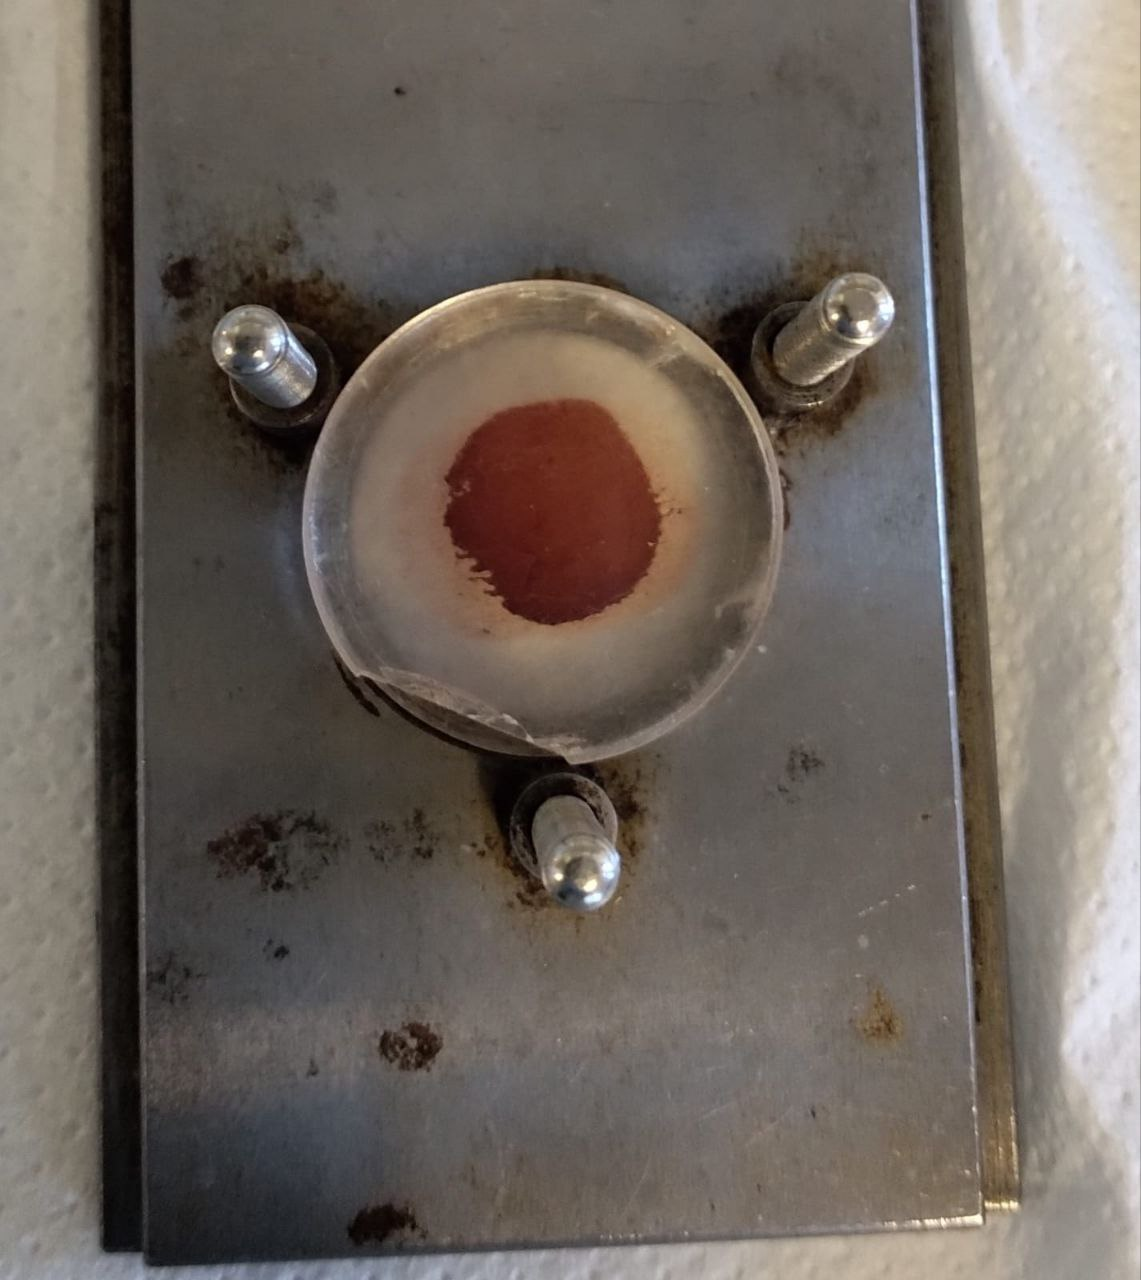
\includegraphics[width=60mm]{Relazione/foto/photo_2023-12-22 14.58.16.jpeg}}
     {Preparazione Co(salen) per IR}
\\
\hline
\end{tabular}
\end{figure}

Ulteriori immagini sono presenti nella cartella \url{https://github.com/mfiaschi5/labinorganica/tree/main/Relazione/foto}
\clearpage



\end{appendix}



\printbibliography